\documentclass{article}\usepackage[]{graphicx}\usepackage[]{color}
%% maxwidth is the original width if it is less than linewidth
%% otherwise use linewidth (to make sure the graphics do not exceed the margin)
\makeatletter
\def\maxwidth{ %
  \ifdim\Gin@nat@width>\linewidth
    \linewidth
  \else
    \Gin@nat@width
  \fi
}
\makeatother

\definecolor{fgcolor}{rgb}{0.345, 0.345, 0.345}
\newcommand{\hlnum}[1]{\textcolor[rgb]{0.686,0.059,0.569}{#1}}%
\newcommand{\hlstr}[1]{\textcolor[rgb]{0.192,0.494,0.8}{#1}}%
\newcommand{\hlcom}[1]{\textcolor[rgb]{0.678,0.584,0.686}{\textit{#1}}}%
\newcommand{\hlopt}[1]{\textcolor[rgb]{0,0,0}{#1}}%
\newcommand{\hlstd}[1]{\textcolor[rgb]{0.345,0.345,0.345}{#1}}%
\newcommand{\hlkwa}[1]{\textcolor[rgb]{0.161,0.373,0.58}{\textbf{#1}}}%
\newcommand{\hlkwb}[1]{\textcolor[rgb]{0.69,0.353,0.396}{#1}}%
\newcommand{\hlkwc}[1]{\textcolor[rgb]{0.333,0.667,0.333}{#1}}%
\newcommand{\hlkwd}[1]{\textcolor[rgb]{0.737,0.353,0.396}{\textbf{#1}}}%
\let\hlipl\hlkwb

\usepackage{framed}
\makeatletter
\newenvironment{kframe}{%
 \def\at@end@of@kframe{}%
 \ifinner\ifhmode%
  \def\at@end@of@kframe{\end{minipage}}%
  \begin{minipage}{\columnwidth}%
 \fi\fi%
 \def\FrameCommand##1{\hskip\@totalleftmargin \hskip-\fboxsep
 \colorbox{shadecolor}{##1}\hskip-\fboxsep
     % There is no \\@totalrightmargin, so:
     \hskip-\linewidth \hskip-\@totalleftmargin \hskip\columnwidth}%
 \MakeFramed {\advance\hsize-\width
   \@totalleftmargin\z@ \linewidth\hsize
   \@setminipage}}%
 {\par\unskip\endMakeFramed%
 \at@end@of@kframe}
\makeatother

\definecolor{shadecolor}{rgb}{.97, .97, .97}
\definecolor{messagecolor}{rgb}{0, 0, 0}
\definecolor{warningcolor}{rgb}{1, 0, 1}
\definecolor{errorcolor}{rgb}{1, 0, 0}
\newenvironment{knitrout}{}{} % an empty environment to be redefined in TeX

\usepackage{alltt}
\usepackage{Sweave}
\usepackage{float}
\usepackage{graphicx}
\usepackage{tabularx}
\usepackage{siunitx}
\usepackage{geometry}
\usepackage{pdflscape}
\usepackage{mdframed}
\usepackage{natbib}
\bibliographystyle{..//refs/styles/besjournals.bst}
\usepackage[small]{caption}
\setkeys{Gin}{width=0.8\textwidth}
\setlength{\captionmargin}{30pt}
\setlength{\abovecaptionskip}{0pt}
\setlength{\belowcaptionskip}{10pt}
\topmargin -1.5cm        
\oddsidemargin -0.04cm   
\evensidemargin -0.04cm
\textwidth 16.59cm
\textheight 21.94cm 
%\pagestyle{empty} %comment if want page numbers
\parskip 7.2pt
\renewcommand{\baselinestretch}{1.5}
\parindent 0pt

\newmdenv[
  topline=true,
  bottomline=true,
  skipabove=\topsep,
  skipbelow=\topsep
]{siderules}

%% R Script


\IfFileExists{upquote.sty}{\usepackage{upquote}}{}
\begin{document}
\title{Rethinking False Spring Risk}
\author{C. J. Chamberlain $^{1,2}$, B. I. Cook $^{3}$, I. Garcia de Cortazar Atauri $^{4}$, E. M. Wolkovich $^{1,2}$}
\date{\today}
\maketitle 
 

\renewcommand{\thetable}{\arabic{table}}
\renewcommand{\thefigure}{\arabic{figure}}
\renewcommand{\labelitemi}{$-$}

%%%%%%%%%%%%%%%%%%%%%%%%%%%%%%%%%%%%%%%%%%%%%%%
\section*{Introduction}
\begin{enumerate}
\item Introduce False Spring Concept
\begin {enumerate}
\item Plants growing in temperate environments are at risk of being exposed to late spring freezes, which can be detrimental to growth. 
\item Individuals that leaf out before the last freeze date are at risk of leaf loss, damaging wood tissue, and slowed or stalled canopy development \citep{Gu2008, Hufkens2012}. 
\item These late spring freezing events are known as false springs. 
\item False spring events can result in highly adverse ecological and economic consequences \citep{Knudson2012, Ault2013}.
\end{enumerate}

\item Introduce Climate Change and Importance of False Spring Studies
\begin{enumerate}
\item Climate change is expected to cause an increase in damage from false spring events around the world due to earlier spring onset and greater fluctuations in temperature \citep{Cannell1986, Inouye2008, Martin2010}. 
\item Temperate forest species around the world are initiating leafout about 4.6 days earlier per degree Celsius \citep{Wolkovich2012, Polgar2014}. 
\item It is anticipated that there will be a decrease in false spring frequency overall but the magnitude of temperature variation is likely to increase, therefore amplifying the expected intensity of false spring events \citep{Kodra2011, Allstadt2015}. 
\item Already, multiple studies have documented false spring events in recent years \citep{Gu2008, Augspurger2009, Knudson2012, Augspurger2013} and some have linked this to climate change \citep{Ault2013, Allstadt2015, Muffler2016, Xin2016}. 
\item Due to these reasons, it is crucial for researchers to properly evaluate the effects of false spring events on temperate forests and agricultural crops in order to make more accurate predictions on future trends.
\end{enumerate}

\item Introduce How Researchers Currently Estimate False Spring (incl. Current False Spring Index Equation)
\begin{enumerate}
\item Growing interest in false spring has led to a lot of research investigating the effects on temperate forests and agricultural crops. 
\item A False Spring Index (FSI) signifies the likelihood of a damage to occur from a late spring freeze. 
\item Currently, FSI is evaluated by the day of budburst and the day of last spring freeze through a simple equation as seen below \citep{Marino2011}. 
\begin{equation} \label{eq:1}
FSI = Julian Date (Last Spring Freeze) - Julian Date (Budburst)
\end{equation}
\item This FSI, however, makes a suite of assumptions, including:
\begin{enumerate}
\item Different species respond the same to late spring freezing events 
\item The level of damage sustained by plants from a false spring is constant across phenophases. 
\end{enumerate}
\item In contrast to these simplifications, we argue that a wealth of factors greatly impacts plants' false spring risk such that simple indices will most likely lead to inaccurate predictions and ultimately do little to advance the field. 
%\item Give quick list here and simple evidence of some of the big factors you will discuss... % not sure how to make this different from the second to last line of the next paragraph. Need to work on!
\end{enumerate}

\item State the Purpose of the Paper
\begin{enumerate}
\item In this paper we aim to highlight the complexity of factors driving a plant's false spring risk. 
\item We outline in particular how life stage of the individual \citep{Caffarra2011}, location within a forest or canopy \citep{Augspurger2013}, winter chilling hours (Flynn \& Wolkovich 2017?), freeze duration/intensity, and range limits of the species \citep{Martin2010} unhinge simple metrics of false spring. 
\item The ultimate intent is to demonstrate how an integrated view of false spring that incorporates these factors would rapidly advance progress in this field.  
\end{enumerate}
\end{enumerate}

%%%%%%%%%% DEFINING FALSE SPRING %%%%%%%%%%%%%

% Possible re-ordering framework %
% (1) How frosts hurt plants (1 paragraph)
% (2) How plants deal with this (include brief discussion of cues for temperate plant leafout): (a) avoidance, (b) tolerance
% (3) How False Spring is currently defined
% (4) Major issues with how False Spring is currently defined: (a) assumes way to much consistency across species, (b) ignore vegetative risk reality

\section*{Defining False Spring}
% Set up spring onset, last freeze date, but many other things matter ... 
\begin{enumerate}
\item Freezing Damage: Quickly review how freezing causes damage 
\begin{enumerate}
\item Temperate forest plants are most at risk to frost damage from episodic spring frosts \citep{Sakai1987}. 
\item Freezing temperatures following a warm spell could result in plant damage or even death \citep{Ludlum1968, Mock2007}.
\item Freeze damage can occur directly via intracellular ice formation or indirectly via freezing dehydration \citep{Pearce2001, Beck2004, Hofmann2015}.
\item Intracellular ice formation can cause defoliation, which can result in crown dieback \citep{Gu2008}. %% There's a point that I would like to make later about how crown dieback from a false spring could cause increased sun exposure to understorey plants meaning false spring events can almost have a domino effect.
\end {enumerate}

\item Current Definition
\begin{enumerate}
\item False springs are defined by two phases: rapid vegetative growth prior to a freeze and a post freeze setback \citep{Gu2008}.
\item Frost damage usually occurs when there is a warmer than average March, a freezing April, and enough growing degree days between budburst and the last freeze date \citep{Augspurger2013}.
\item A damaging false spring is currently defined as having 7 or more days between budburst and the last freeze date (Equation \ref{eq:1}) \citep{Peterson2014}.
\item The 7 day parameter exposes less resistant foliate phenophases to a false spring, thus putting the plant at a higher risk of damage. 
\item Once budburst has initiated, buds cannot respond to cold temperatures and freeze resistance is greatly reduced \citep{Taschler2004, Lenz2013, Vitasse2014}.
\end{enumerate}
\end{enumerate}

%Re-WORK this to move out any specifics on seedlings/saplings etc. (anything that gets at variation) ... 
\section*{Determining Spring Onset and Last Freeze Date in Temperate Plant Communities}
\begin{enumerate}
\item Elucidate the difference between spring onset and study species 
\begin{enumerate}
\item Spring phenology in temperate forests typically progresses by functional group: understory species and young trees tend to initiate budburst first, whereas late successional species may start later in the season \citep{Richardson2009, Xin2016}.
\item False spring studies should first assess the forest demographics and functional groups of the study species in order to effectively estimate the date of spring onset.

\end{enumerate}
%%%%%%%%%%%%%% MOVE SWIFTLY!!! %%%%%%%%%%%%%%%%%%%%%%%%
%%%%%%%%%%%%%%%%%%%%%%%%%%%%%%%%%%%%%%%%%%%%%%%%%%%%%%%
%{\textbf Okay, we apply this definition to some datasets .... but they differ! Why? Because species differ}
%%%%%%%%%% DETERMINING SPRING ONSET in temperate plant communities %%%%%%%%%%%%%
% Focus on species groupings (like functional types etc.?) and then more on individual species ... 
%% Maybe start with equation and the two inputs then break down why spring onset can't be defined and that last freeze date is uncertain

\item Methodologies: False spring is defined dependent on metholodology for onset, make sure your methodology matches your question 
\begin{enumerate}
\item A suitable methodology for determining spring onset is crucial in order to establish an effective model for false spring risk, especially since the current false spring equation only uses two inputs: date of spring onset and date of last freeze (Equation \ref{eq:1}). 
%\item If the date of spring onset is inaccurate, the level of risk determined by the current equation (Equation \ref{eq:1}) could render erroneous results. 
%\item There are many methods available to ascertain the first day of spring.
\item Spring onset can be calculated through observational data, PhenoCam or remote-sensing data, or through the USA National Phenology Network's (USA-NPN) Extended Spring Index (SI-x) tool \citep{USA-NPN2016}.
\item These three methodologies were compared using observational data from Harvard Forest \citep{Okeefe2014}, PhenoCam data from Harvard Forest \citep{Richardson2015}, and USA-NPN SI-x \citep{USA-NPN2016} and then inputted into the FSI equation (Equation \ref{eq:1}) to calculate FSI values from 2008 to 2014 (Figure \ref{fig:fsifig}).
% Short example paragraph below %
\item In 2012, a false spring event was reported through many regions of the US due to warm temperatures occurring in March \citep{Ault2015}.
\item These high temperatures would most likely be too early for larger canopy species to initiate budburst but they would affect smaller understory species as is seen by the discrepancy in results for 2012 (Figure \ref{fig:fsifig}).
\item The risk of a false spring varies across habitat type and species composition since spring onset is not consistent across functional groups.
\item Therefore, one spring onset date cannot be used as an effective proxy for all species. % One point that I would like to make over the course of the paper is that these smaller species are opportunistic now and are willing to take the false spring risk, but with spring advancing and last freeze date staying the same, these little guys are no longer taking that risk, the big guns are, which could be really shocking to the canopy folks and potentially severely detrimental to the entire system. 
\end{enumerate}

% Two versions - one after "we apply this to some datasets" (reiterate, be more clear to species) and here -Now we say, but WAIT! All this assumes plants as a monolith, when the reality is much more complex based on basic physiology and based on species differences 
\item Major Issues with Current Definition
\begin{enumerate}
\item The current definition of a false spring also fails to incorporate the different avoidance and tolerance strategies commonly seen in temperate forest species.
\item The FSI equation and 7 day parameter assumes consistency across species, functional group, life stage, habitat type, and other climatic regimes, which is largely inadequate. 
\item A new approach that integrates these other crucial factors is necessary to accurately determine current false spring damage and future spring freeze risk. 
\end{enumerate}
\end{enumerate}

\section*{Plant physiology and diversity versus current FS definition}
\begin{enumerate}
\item Avoidance and Tolerance of False Springs: Understanding how species avoid/tolerate false springs 
\begin {enumerate}
% One paragraph on avoidance 
\item Plants have evolved multiple strategies to avoid false springs, which must be considered in any false spring definition.
\item Temperate deciduous tree species optimize growth and minimize spring freeze damage by using three cues to initiate budburst: low winter temperatures, warm spring temperatures, and longer photoperiods \citep{Cleland2007, Polgar2011} (Figure \ref{fig:cues}).

%%%%%%%%%%%%%% COME BACK TO THIS!!! %%%%%%%%%%%%%%%%%%%%%%%%%%%
\item Deciduousness and the evolution of dormancy in temperate forest trees has permitted species to occupy more northern ecological niches and decrease the risk of false spring damage \citep{Samish1954}.
\item Therefore, warm temperatures earlier in the year (i.e. in February) will not result in early budburst due to insufficient chilling \citep{Basler2012}.
\item Likewise, photoperiod sensitivity is a common false spring avoidance strategy: species that respond to photoperiod cues more than warm spring temperatures will likely delay budburst and evade false spring events (as spring continues to advance earlier in the year) \citep{Basler2014}.
\end {enumerate}
\item Tolerance
% One paragraph on tolerance 
\begin{enumerate}
\item Some temperate forest species have evolved to be more tolerant of spring freezing temperatures.
\item Temperate forest plants utilize various morphological strategies to be more frost tolerant: some have toothed or lobed leaves to increase `packability' in winter buds \citep{Edwards2017}, others have young leaves with more trichomes to act as a buffer against spring frosts \citep{Agrawal2004}, and many are able to respond to environmental cues such as dry winters. 
\item Dry winters typically result in new, frost-tolerant shoots due to the decreased water content and osmotic potential from the reduced number of accumulated solutes \citep{Morin2007, Hofmann2015}.
\item It is hypothesized that increased bud dehydration results in increased frost hardiness \citep{Beck2007, Nielsen2009, Poirier2010, Kathke2011, Hofmann2015}.
\item More studies are needed to investigate the interplay between false spring events, leaf morphology, and precipitation and how these relationships affect false spring tolerance.
\end{enumerate}
\end{enumerate}



%%%%%%%%%% Understanding (Defining?) Vegetative Risk %%%%%%%%%%%%%
% Keep working in species differences, now add in phenophases and return to concept of tolerance .... 
\section*{Defining Vegetative Risk} % This section maybe needs species differences somewhere else? 
%%%%% Maybe keep species differences here because the two figures we use incorporate climate change a lot, which is also heavily tied into species differences? Not sure... still thinking through it %%%%%%%%
\begin{enumerate}
\item Species Differences: They matter 
\begin {enumerate}
\item Different species respond differently to anthropogenic climate change.
\item Most species are expected to begin leafout earlier in the season with warming spring temperatures but some species may have the opposite response \citep{Cleland2006, Yu2010, Xin2016}.
\item Studies indicate that species growing at more northern latitudes tend to respond greater to photoperiod than species growing further south \citep {Partanen2004, Viheraaarnio2006, Caffarra2011}.
\item Similarly, late successional species exhibit greater photoperiod sensitivities than pioneer or understory species \citep{Basler2012} and they also require more chilling in the winter and greater forcing temperatures in the spring to initiate budburst \citep{Laube2013}.
\item It is anticipated that these more opportunistic individuals that initiate budburst earlier in the spring would attempt to limit freezing risk by increasing the rate of budburst and progress to full leaf expansion faster.
\end{enumerate}

\item Phenophase Differences: They matter 
\begin {enumerate}
\item Reproductive phases are generally more sensitive to false spring events than vegetative phases. \citep{Augspurger2009, Lenz2013}.
\item However, false spring events that occur during the vegetative growth phenophases impose the greatest freezing threat to deciduous tree and shrub species because plants will suffer greater long-term effects from the loss of photosynthetic tissue than trees that lose one year of reproductive growth \citep{Sakai1987}.
\item Plants at certain vegetative phenophases (i.e. before full leafout of the entire plant) are more likely to sustain damage from a false spring than individuals past the leafout phenophase. 
\item Spring phenology is a crucial indicator for how much damage a plant will sustain from a freezing event.
\end {enumerate}

\item Frost Tolerance
\begin{enumerate}
\item Freezing tolerance steadily decreases after budburst begins until the leaf is fully unfolded \citep{Lenz2016}.
\item Therefore, the rate of budburst and the length of time between budburst and leafout is essential for predicting level of damage from a false spring event.
\item We will refer to the timing of these collective phenophases (i.e. budburst to leafout) as the duration of vegetative risk.
\item The duration of vegetative risk is usually extended if a freezing event occurs during the phenophases between budburst and full leafout.
\item Species with short durations of vegetative risk often sustain higher levels of damage \citep {Augspurger2009}.
\item It is hypothesized that if the duration of vegetative risk is longer, then the buds and leaves will be heartier against frosts, however this has yet to be tested thoroughly.
\item We assess the interaction between duration of vegetative risk and false spring events using two datasets: from long-term observational data and a growth chamber chilling experiment.
% Set up below or here or both places, connections to climate change
\end {enumerate}


% Could move up Harvard Forest, which is about FORCING and near-term climate change impacts 
% Then talk about Dan's data as Forcing X photo X chilling  ... and longer-term nonlinearities with climate change 
%%% Should I talk more about oscillating temperatures or cut that part? %%%%%

%%%% REFINE DAN'S and HF! Keep cleaning! %%%%%%
%%%%%%%%%%%%%% KEEP WORKING!!!! - 13 JULY CAT %%%%%%%%%%%%%%%%%%
\item Harvard Forest Data: Climate change may be similar to an earlier year -- susceptibility to multiple freezes 
\begin{enumerate}
\item Tell the forcing temperature story
\begin{enumerate}
\item Forcing temperatures in the spring affect the duration of vegetative risk: years with lower forcing temperatures and fewer growing degree days will have longer durations of vegetative risk \citep{Donnelly2017}.
\item With spring advancing, it is anticipated that there will be greater fluctuations in spring forcing temperatures \citep{Martin2010}.
\item This high variation in temperature (i.e. oscillating above and below the development threshold) may result in longer durations of vegetative risk across more species.
\item Using observational data from Harvard Forest \citep{Okeefe2014}, we compared two years of data: one year that had an unusually early spring onset (2010) and another year that an unusually late spring onset (2014).
\end{enumerate}
\item Harvard Forest Data
\begin{enumerate}
\item By comparing the durations of vegetative risk to the growing degree days for each year, we found that the number of growing degree days were highly comparable for both years, however, in 2010, the duration of vegetative risk was slightly longer overall (Figure \ref{fig:forest}). 
\item With climate change progressing, it is likely there will be more years like 2010 in the future and that the durations of vegetative risk will continue to extend. %% can expand later 
\item Therfore, species that are better able to phenologically track the shifts in spring advancement due to climate change are more likely to sustain damage from false springs \citep{Scheifinger2003}.
\end{enumerate}
\end{enumerate}


%%%%%%%%%%%%% NEEDS TO BE WORKED ON! %%%%%%%%%%%%%%%%%%%%%
\item Dan's Data: Take home messages: Wraps back to physiology and answers questions about how those cues impact bb and leafout and how it varies by species *and* also, gives us insight into what climate change may alter
\begin{enumerate}
\item Tell the interaction of cues story
\begin{enumerate}
\item Spring forcing temperatures and daylength requirements for budburst to occur vary among species and habitats.
\item Since species distributions are largely driven by phenology \citep{Chuine2001}, species less reliant on photoperiod cues are likely to outcompete species that are reliant on photoperiod cues as spring forcing temperatures continue to initiate earlier \citep{Vitasse2011, Gauzere2017}.
\item As climate change progresses, higher spring forcing temperatures may be required due to potentially insufficient winter chilling, especially at lower latitudes \citep{McCreary1990, Morin2009, Fu2012, Polgar2014, Chuine2010}. 
\item Anthropogenic climate change will cause changes in winter and spring temperatures, resulting in greater differences in spring phenology cue requirements across species and habitats. 
\item This interaction of cues and how climate change will affect that interaction is crucial to understand in order to recognize the species that will be affected and to understand which species will likely become more at risk of false spring events in the future. 

\end{enumerate}


\item The Experiment Data
\begin{enumerate}
\item Data from a growth chamber experiment were used to compare 9 temperate forest species between two treatments: high chilling hours, long photoperiod and high forcing temperatures (WL1) against no additional chilling, short photoperiod and low forcing temperatures (CS0) (Flynn and Wolkovich, 2017?).
\item According to the results, individuals that initiate budburst earlier in the season (i.e. {\textit {Betula papyrifera}} (Marsh.) and {\textit{Ilex mucronata}} (L.)) tend to initiate budburst early regardless of treatment, but the treatment does affect the duration of vegetative risk significantly (Figure \ref{fig:dan}).
\item As the season progresses, treatment does not affect the duration of vegetative risk as much but the day of budburst tends to be later in the season with the weaker treatment effects (i.e. CS0).
\item Anova results indicate forcing temperatures and photoperiod length determine the duration of vegetative risk more than chilling requirements.
\item This could suggest that chilling influences budburst and leafout similarly, while photoperiod and forcing temperatures have varying effects on the two phenophases.
\item With a changing climate, forcing temperatures will increase while photoperiod cues will remain stagnant, potentially elongating the duration of vegetative risk and exposing at risk plants to more intense false spring events or even multiple events in one year. %% NEEDS FIXING!!
\item Further studies are essential to investigate the interplay between chilling, forcing, and photoperiod cues on the duration of vegetative risk, especially for species occupying ecological niches more susceptible to false spring events. 
\end{enumerate}
\end {enumerate}
\end{enumerate}

%%%%%%%%%%%%%%%%%%%% Regional Differences in False Spring Risk %%%%%%%%%%%%%%
%Transition here: False springs and species cues beyond two New England datasets (above): We need to extrapolate this thinking across regions  ... \\
%Latitude matters (photoperiod) -- some focus on this already \\
%But, we know forcing and chilling also matters -- so that means climate regime extremes (annual minima, maxima) and amplitude/variation during winter/spring matters (continental/coastal)\\
%Here we show this somewhat ....\\
%We should be working towards to better predictions! \\
\section*{Predictable Regional Differences in False Spring Risk and Temperature Thresholds}
\begin{enumerate}
\item Introduce concept of regional differences
\begin {enumerate}
\item There have been numerous studies investigating the relationship between budburst and photoperiod by using latitudinal gradients \citep{Partanen2004, Viheraaarnio2006, Caffarra2011, Zohner2016, Gauzere2017}, however most studies fail to integrate longitudinal variation or regional effects.
\item Chilling and forcing are key drivers of budburst and leafout and can vary significantly across a  longitudinal gradient while maintaining the same photoperiodic effects. %% needs some work!
\item Climatic variation across regions results in varying durations of vegetative risk due to different chilling and forcing temperatures.
\item For this reason, it is important to include climate regime extremes (e.g. annual minima and annual maxima) in future studies.
\item It is essential to recognize the differences in continental vs. coastal habitats and the amplitude and variation in temperature extremes across regions in order to properly assess spring plant phenology and false spring risk.
\end{enumerate}
\item Regional differences and Risk more in depth
\begin{enumerate}
\item The climatic implications of advancing forcing temperatures could potentially lead to earlier dates of budburst and enhance the risk for frost or drought risk.
\item These shifts in climatic regimes could vary in intensity across regions (i.e. habitats currently at risk of false spring damage could become low risk regions over time). 
\item There are discrepancies in defining a false spring event, especially with understanding damaging freezing temperatures.
\item Some regions and species may be more able to tolerate lower temperature thresholds than others (Table \ref{tab:temperature}).
\item It is crucial to gain an understanding on which climatic parameters result in false spring events and how these parameters may vary across regions. 
\item It is anticipated that most regions will have earlier spring onsets, however, last freeze dates will not occur at the same rate, rendering some regions and species to be more susceptible to false spring events in the future \citep{Labe2016}.
\item By determining the average time of budburst to leafout dates for the dominant species in five archetypal climate regions, we were able to estimate the current spatial variation of false spring risk (Figure \ref{fig:regional}).
\item We assessed the number of freeze days (-2.2$^{\circ}$C) \citep{Schwartz1993} that occurred on average over the past 50 years within the date ranges for each region.
\item We found that Maine has the highest risk for frost damage and Lyon, France as the lowest (Figure \ref{fig:regional}). 
\item Future research should aim to integrate spatiotemporal effects and regional differences when investigating false spring risk in order to make better predictions as climate change progresses.
\end {enumerate}
\end{enumerate}

%%%%%%%%%%%%%%%%%%%%% DISCUSSION AND CONCLUSION %%%%%%%%%%%%%%%%%%%%%%%%%%%%%%%%%%%%%%%%%%%

\section*{Conclusion}
\begin{enumerate}
\item Significance of False Spring events
\begin{enumerate}
\item As global change progresses and atmospheric CO$_{\text{2}}$ increases, false spring damage will likely worsen and low temperature thresholds will decrease (Table \ref{tab:temperature}) \citep{Beerling2001, Barker2005}.
\item Plants have higher freeze tolerance after exposure to low temperatures over a period of time \citep{Thomashow1999} so shorter dormancy lengths coupled with elevated CO$_{\text{2}}$ levels could result in highly adverse effects. 
\item Ecosystem dynamics and risk of damage can vary from year to year and the timing between last freeze date and date of spring onset may become less consistent. 
\item With warm temperatures advancing in the spring but last spring freeze dates staying the same, there could potentially be more damaging events in the future, especially in high risk regions \citep{Gu2008, Inouye2008}.
\item This shift in timing could result in more events where understory species leaf out prior to the last freeze and escape frost damage but canopy species may be at higher risk, thus potentially resulting in crown dieback for the larger tree species and subsequently enhanced sun exposure and damage to understory species.
\item False spring events could also adversely affect other trophic levels if fruit and seed development is impacted \citep{Gu2008}, making false spring studies even more ecologically significant.
\end{enumerate}

\item Introduce Phenology
\begin{enumerate}
\item Phenology is closely linked to climatic regimes \citep{Wolkovich2011} and is a key indicator in phenotypic variation for cold adapted traits and false spring risk avoidance.
\item Understanding the variation of spring onset across regions and within habitats as well as the rate of budburst will permit greater insight into false spring risk.
\item Tree species with smaller and more fragmented distribution ranges are more at risk to stochastic events (i.e. frost and drought) \citep{Alberto2013}. 
\item Therefore, it is essential that temperate forest tree species maintain continuous ranges in order to successfully track the changes in climate and to utilize photoperiodic and temperature cues simultaneously rather than rely strictly on photoperiodism especially along range edges \citep{Zohner2016, Gauzere2017}.
\item Future studies are necessary to investigate the relationship between anthropogenic climate change, spatiotemporal factors, the duration of vegetative risk, and the level of damage sustained from false spring events
\end{enumerate}

\item Drive home importance of new equation
\begin{enumerate}
\item By utilizing only two simple metrics (last freeze date and spring onset date), researchers fail to assess the myriad of factors essential in determining false spring risk and damage. 
\item Future studies are necessary to gain an understanding with relationships between species, functional group, phenophase, and region and the differences in false spring damage. 
\item It is also essential that a temperature threshold is established for all functional types and phenophases across regions in order to effectively predict false spring risk in the future.
\item An integrated approach to assessing past and future spring freeze damage must be realized as global climate change progresses in order to mitigate the adverse ecological and economic effects of false springs.
\end{enumerate}
\end{enumerate}



\bibliography{..//refs/SpringFreeze.bib}

\begin{figure}[H]
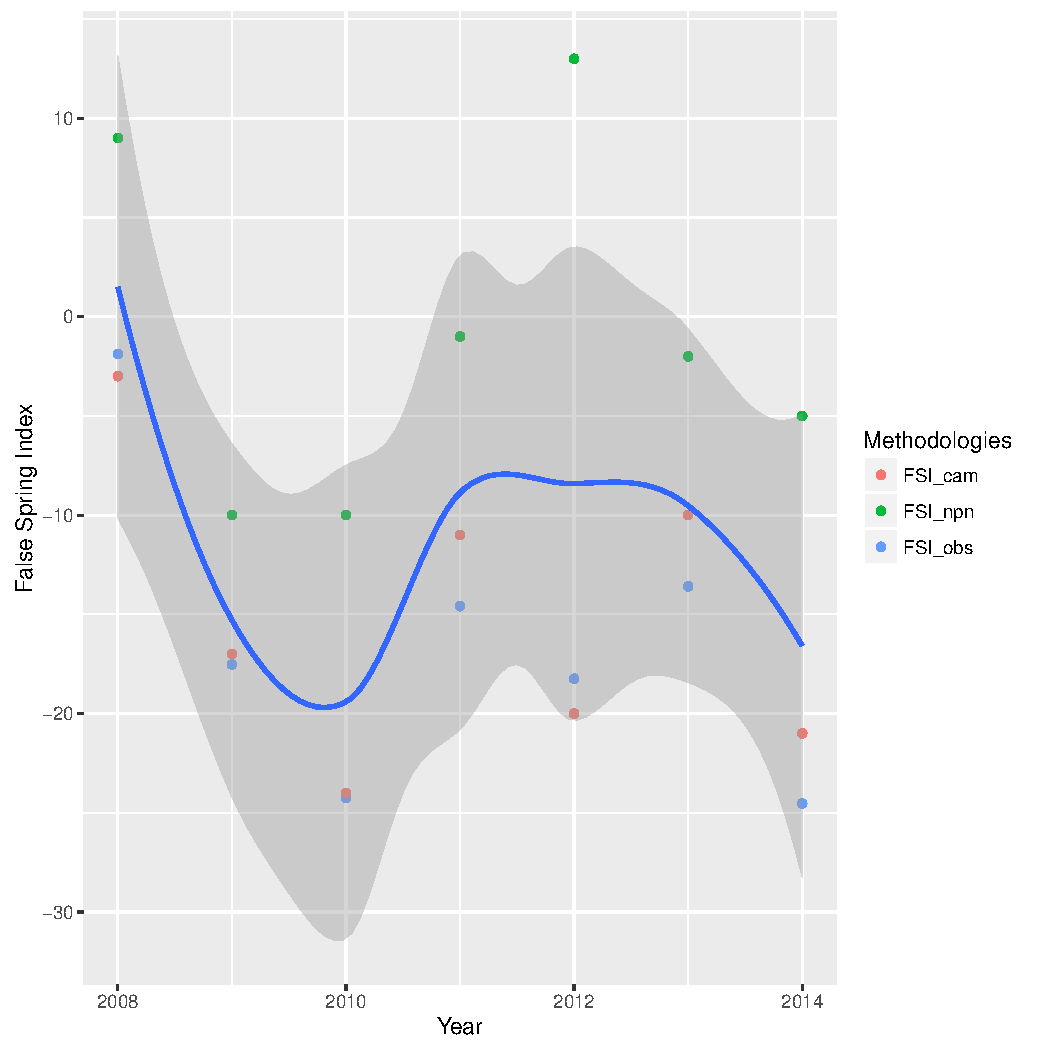
\includegraphics[width=\maxwidth]{figure/fsifig-1} \caption[A scatterplot indicating FSI values from 2008 to 2014 for each methdology used in this study]{A scatterplot indicating FSI values from 2008 to 2014 for each methdology used in this study. PhenoCam FSI values are red, Observed FSI values are blue, and USA-NPN FSI values are green.}\label{fig:fsifig}
\end{figure}



\begin{figure}[H]
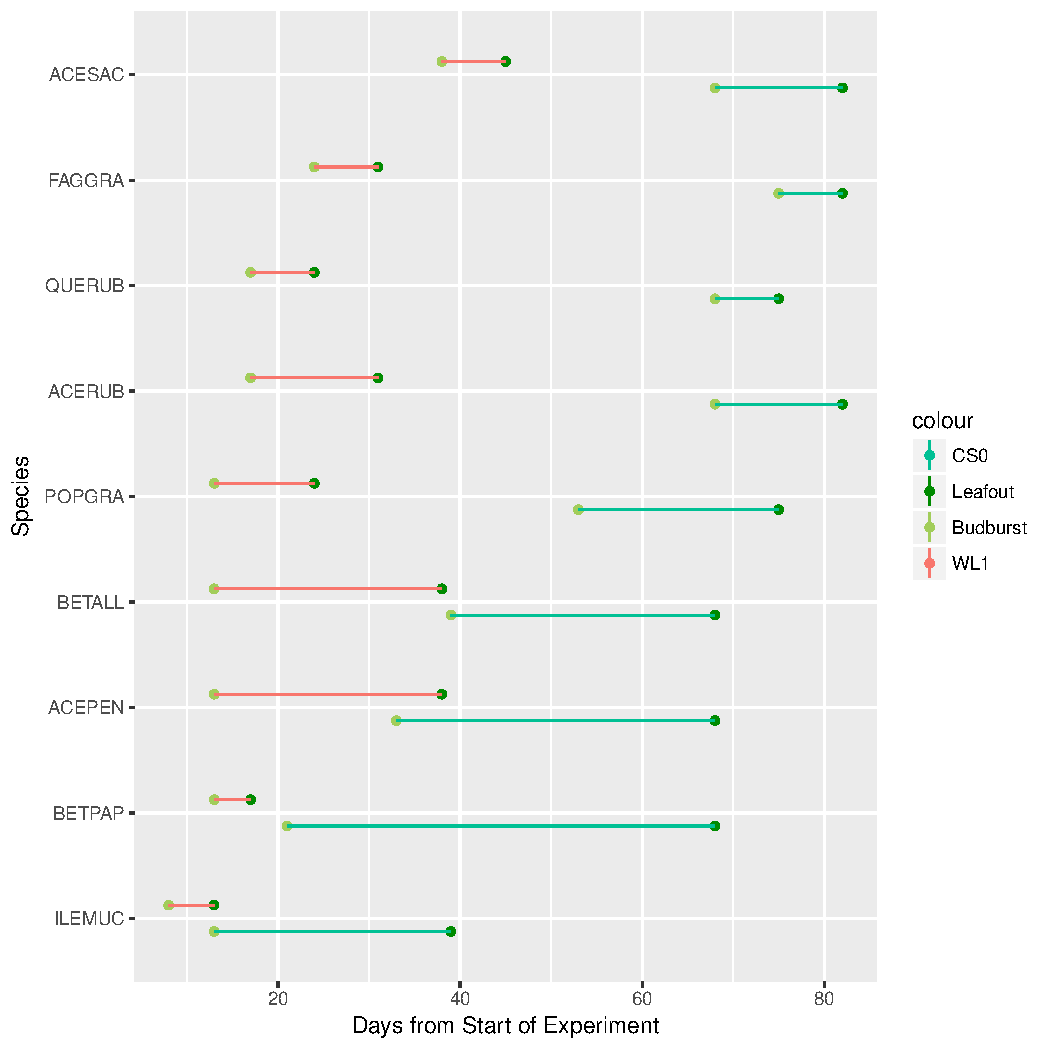
\includegraphics[width=\maxwidth]{figure/dan-1} \caption[Day of budburst and the day of leaf out for native tree species in New England]{Day of budburst and the day of leaf out for native tree species in New England. Data was collected from a growth chamber experiment using any combination of two photoperiod treatments, two forcing treatments, and three chilling treatments. The standard deviation is represented in blue for budburst and green for leaf out.}\label{fig:dan}
\end{figure}



\begin{figure} [H] 
\begin{center}
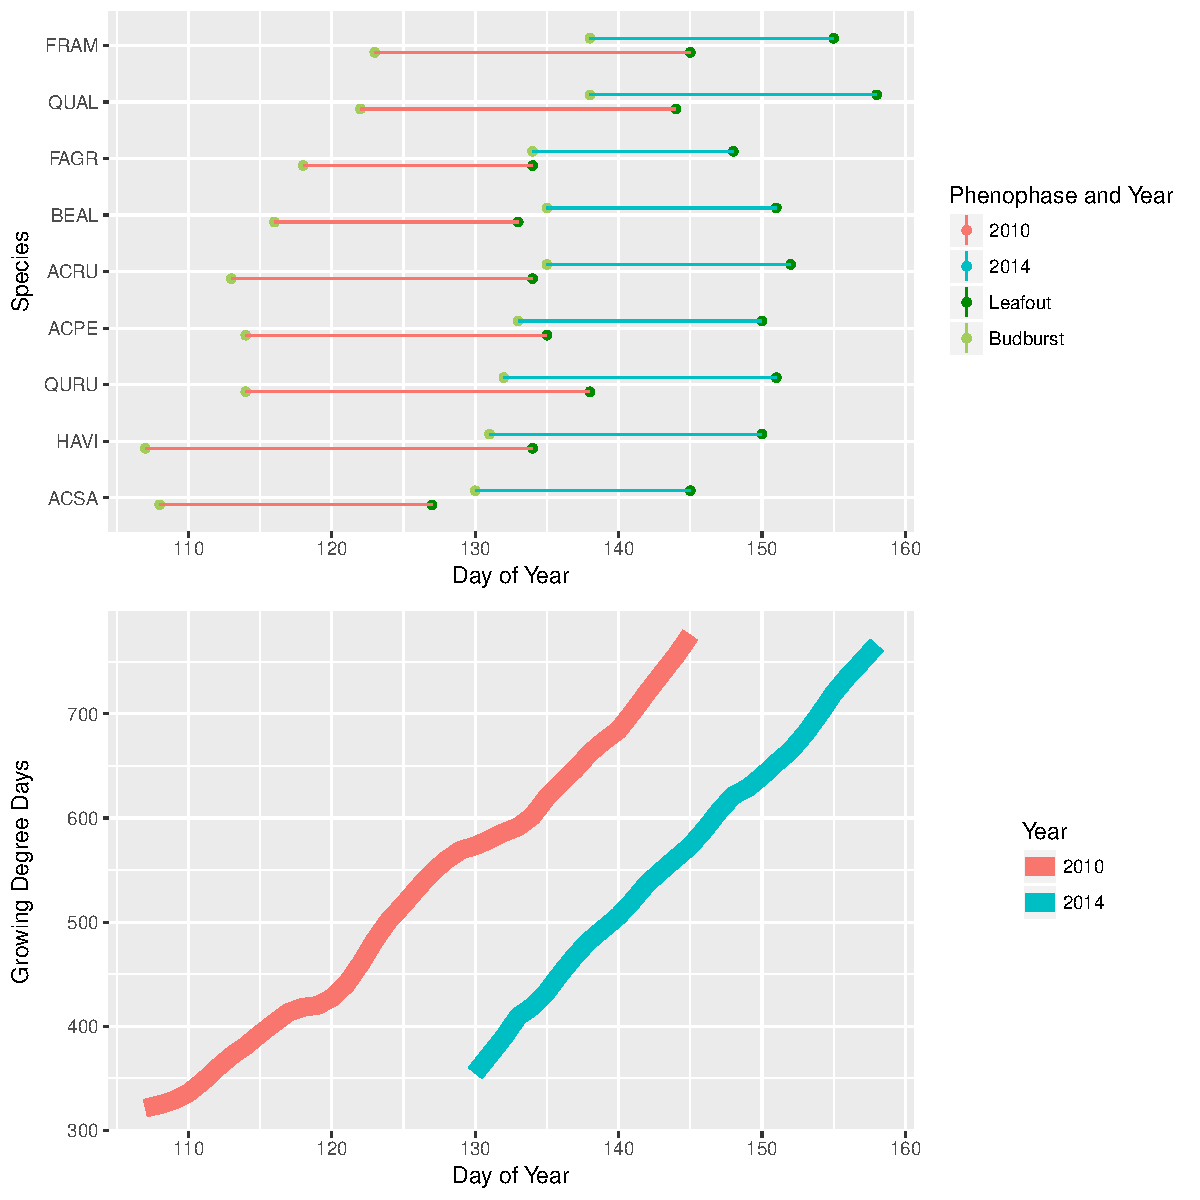
\includegraphics{..//figure/HF_gddTime.pdf}
\caption{A comparison of two years of observational data investigating the effects of growing degree days on the duration of vegetative risk. The average duration of vegetative risk for 2010 was 21 +/- 3.39 days versus 17.1 +/- 1.96 days in 2014.}\label{fig:forest}
\end{center}
\end{figure}

\begin{figure} [H] 
\begin{center}
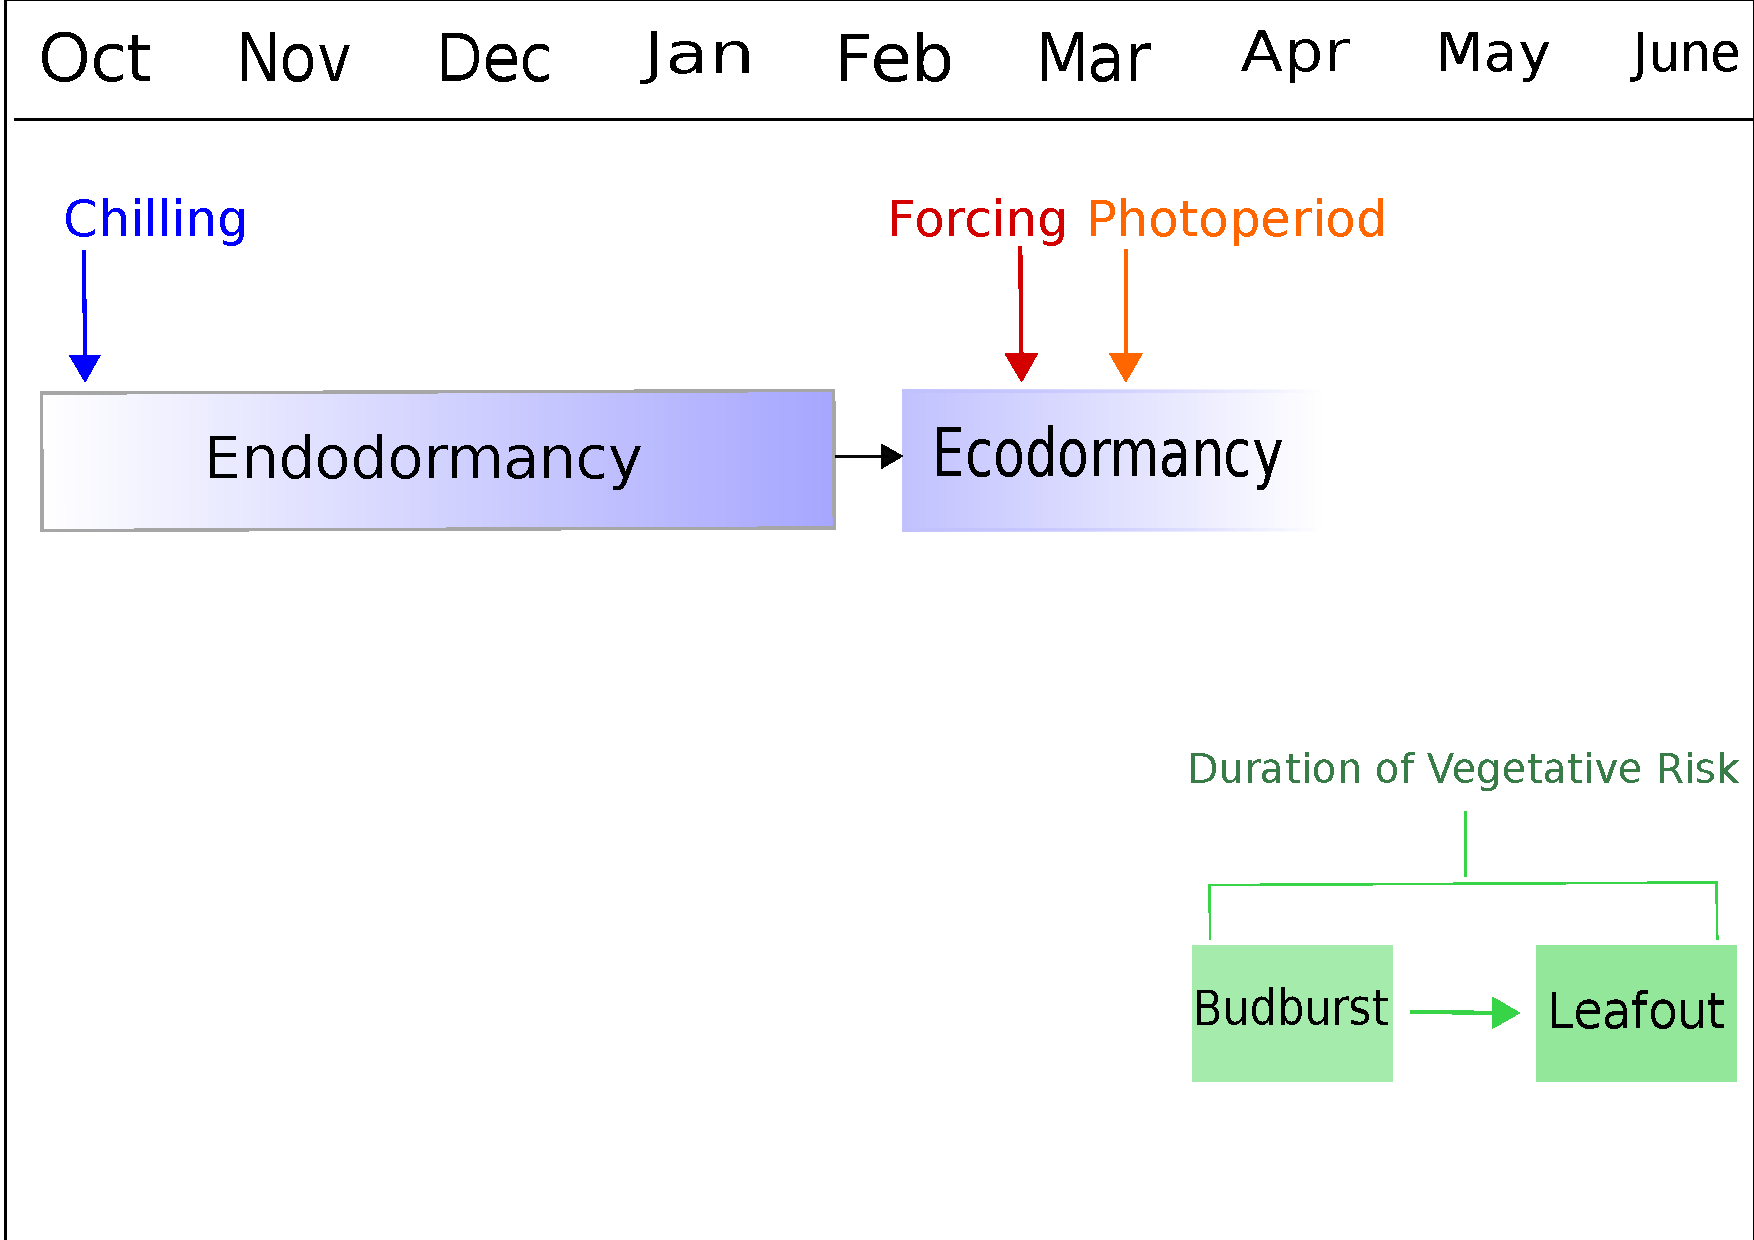
\includegraphics{..//figure/CuesAndFS.pdf}
\caption{Temperate forest trees utilize three main drivers to induce budburst in the spring: chilling over the winter, forcing temperatures in the spring, and longer photoperiod cues. During the endodormancy phase, individuals accumulate chilling hours and cannot break dormancy and false springs cannot occur during the this time. During the ecodormancy phase, however, false spring damage can occur. Damage from a false spring increases as the season progresses, however the likelihood of an event decreases.}\label{fig:cues}
\end{center}
\end{figure}


\begin{landscape}
\begin{center}
\captionof{table}{Comparing damaging spring temperature thresholds in ecological and agronomical studies across various species and phenophases.} \label{tab:temperature} 
\footnotesize
\begin{tabular}{|c | c | c | c | c | c|}
\hline
\textbf{Sector} & \textbf{BBCH} & \textbf{Species} & \textbf{Temperature ($^{\circ}$C)} & \textbf{Type} & \textbf{Source} \\
\hline
Ecological & 9-15 & Sorbus aucuparia & -7.4 & 50\% lethality & \cite{Lenz2016} \\
\hline
Ecological & 9-15 & Prunus avium & -8.5 & 50\% lethality & \cite{Lenz2016} \\
\hline
Ecological & 9-15 & Tilia platyphyllos & -7.4 & 50\% lethality & \cite{Lenz2016} \\
\hline
Ecological & 9-15 & Acer pseudoplatanus & -6.7 & 50\% lethality & \cite{Lenz2016}\\
\hline
Ecological & 9-15 & Fagus sylvatica & -4.8 & 50\% lethality & \cite{Lenz2016}\\
\hline
Ecological & 9+ & All & -2.2 & hard & \cite{Schwartz1993}\\
\hline
Ecological & 9+ & All & -1.7 & soft & \cite{Augspurger2013} \\
\hline
Ecological & All & All & 2 SD below winter TAVG & cold-air outbreaks & \cite{Vavrus2006} \\
\hline
Ecological & 9+ & Eucalyptus pauciflora & -5.8 & elevated CO2 and temperature threshold & \cite{Barker2005} \\
\hline
Ecological & 9+ & All & -2.2 & 7 day threshold & \cite{Peterson2014} \\
\hline
Agrinomical & 9+ & All & 2 & Risk threshold for clear nights & \cite{Cannell1986} \\
\hline
Agrinomical & Floral & Vaccinium spp. & -4.4 to 0 & sprinkler protection threshold & \cite{Longstroth2012} \\
\hline
Agrinomical & 9 & Rosaceae & -7.2 & 10\% lethality & \cite{Longstroth2013}\\
\hline
Agrinomical & 9 & Rosaceae & -13.3 & 90\% lethality & \cite{Longstroth2013} \\
\hline
Agrinomical & All & All & Varies & Radiation Frost & \cite{Barlow2015} \\
\hline
Agrinomical & Floral & Wheat & -4 to -5 & 10-90\% lethality & \cite{Barlow2015} \\
\hline
Agrinomical & Vegetative & Wheat & -7 for 2hrs & 100\% lethality & \cite{Barlow2015} \\
\hline
Agrinomical & Vegetative & Rice & 4.7 & lethal limit & \cite{Sanchez2013} \\
\hline
Agrinomical & Vegetative & Corn & -1.8 & lethal limit & \cite{Sanchez2013}\\
\hline
Agrinomical & Vegetative & Wheat & -17.2 & lethal limit & \cite{Sanchez2013} \\
\hline
\end{tabular}
\end{center}
\end{landscape}
\restoregeometry

\begin{figure} [H] 
\begin{center}
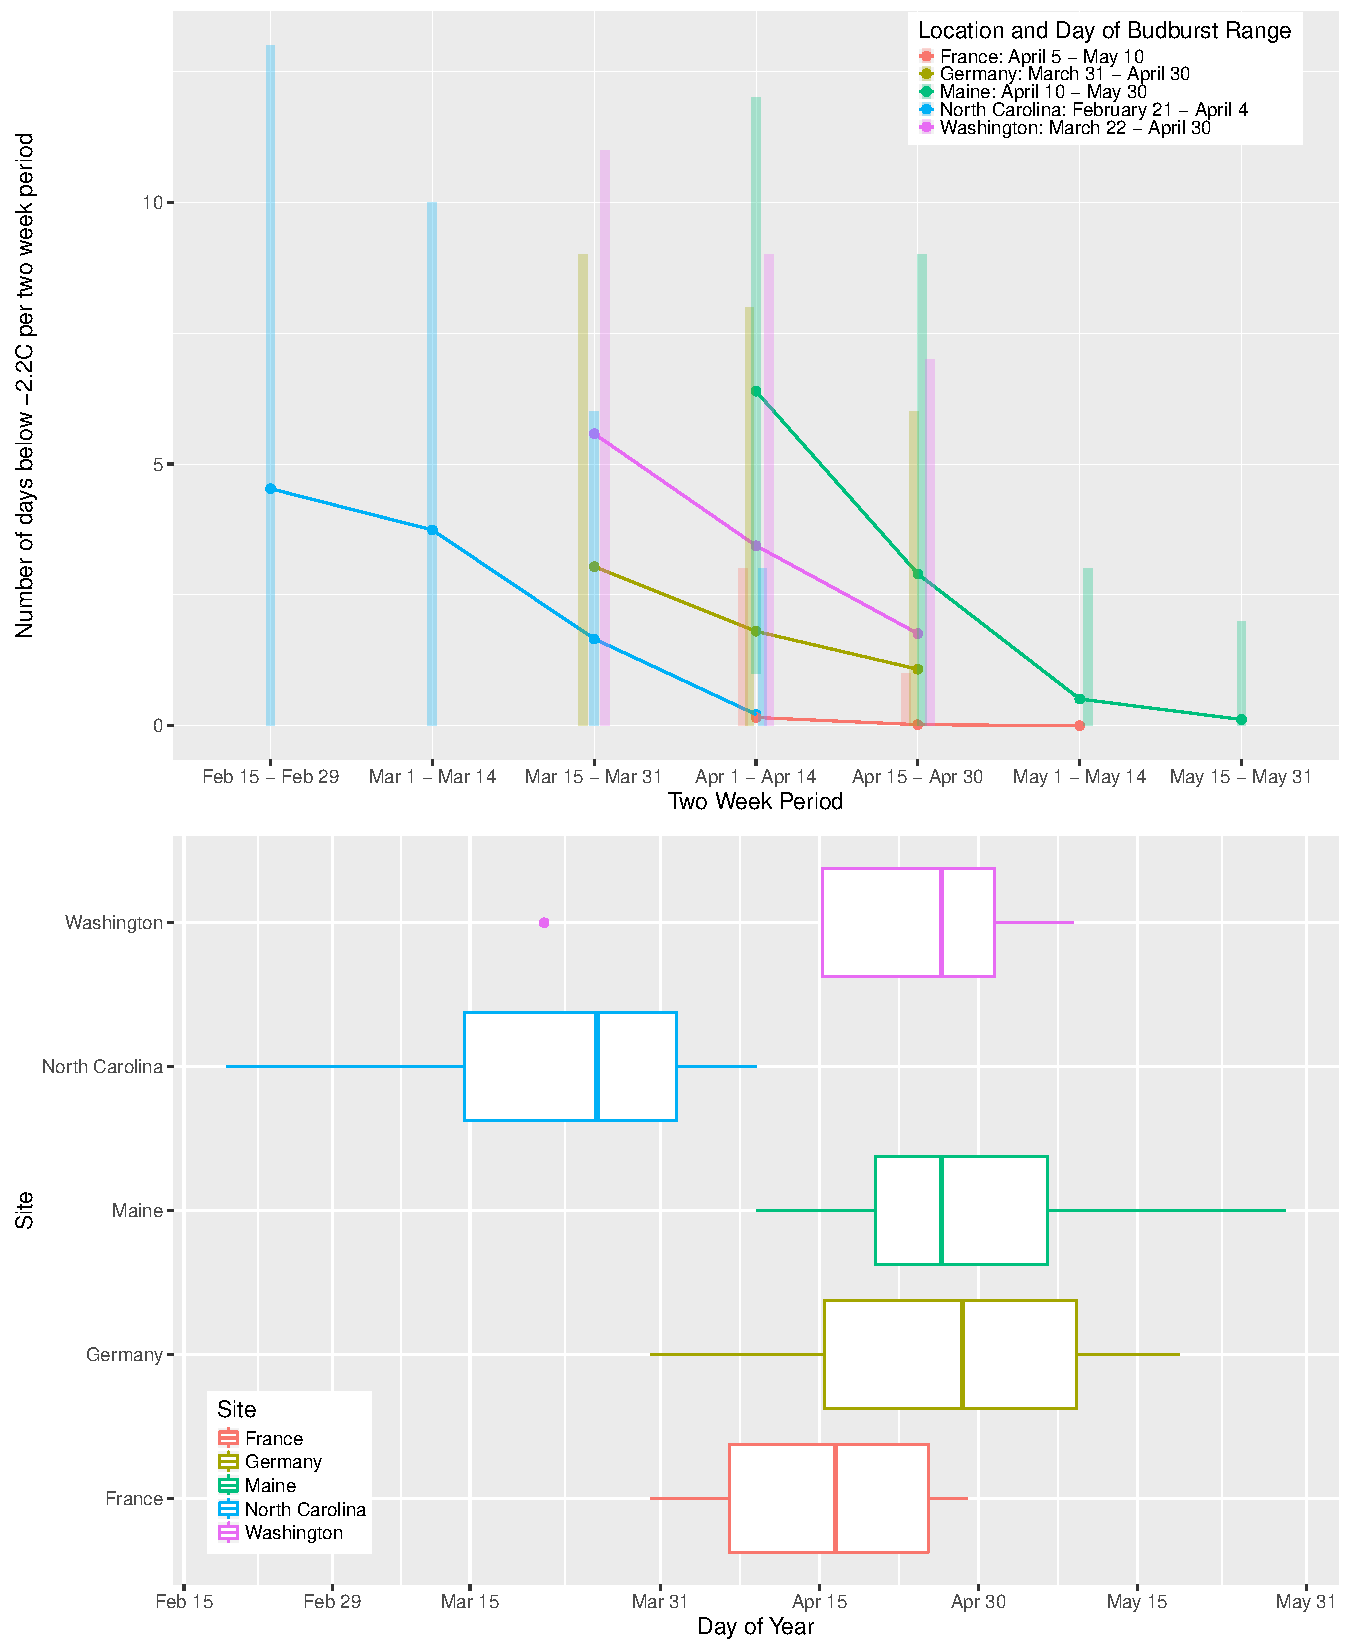
\includegraphics[width=16cm, height=13cm]{..//figure/RegionalRisk.pdf} 
\caption{A comparison of false spring risk across five climate regions. The data was subsetted for each region based on earliest historical spring onset date to the latest historical leafout date and was divided into biweekly time periods \citep{Schaber2005, White2009, Soudani2012, USA-NPN2016}.}\label{fig:regional} 
\end{center}
\end{figure}




\section*{Supplemental Information}
% latex table generated in R 3.3.1 by xtable 1.8-2 package
% Mon Jul 17 08:48:00 2017
\begin{table}[ht]
\centering
\begin{tabular}{rrrrr}
  \hline
  ACEPEN & Sum.Sq & Df & F value & Pr(>F) \\
 \hline
chilling & 149.41 &   2 & 1.20 & 0.30 \\ 
  forcing & 4909.59 &   1 & 78.94 & 0.00 \\ 
  photoperiod & 1309.59 &   1 & 21.06 & 0.00 \\ 
  Residuals & 6654.56 & 107 &  &  \\ 
   \hline
\end{tabular}
\end{table}
% latex table generated in R 3.3.1 by xtable 1.8-2 package
% Mon Jul 17 08:48:00 2017
\begin{table}[ht]
\centering
\begin{tabular}{rrrrr}
  \hline
  ACERUB & Sum.Sq & Df & F value & Pr(>F) \\
 \hline
chilling & 0.62 &   2 & 0.00 & 1.00 \\ 
  forcing & 1731.00 &   1 & 25.92 & 0.00 \\ 
  photoperiod & 462.78 &   1 & 6.93 & 0.01 \\ 
  Residuals & 6611.17 &  99 &  &  \\ 
   \hline
\end{tabular}
\end{table}
% latex table generated in R 3.3.1 by xtable 1.8-2 package
% Mon Jul 17 08:48:00 2017
\begin{table}[ht]
\centering
\begin{tabular}{rrrrr}
  \hline
  ACESAC & Sum.Sq & Df & F value & Pr(>F) \\
 \hline
chilling & 65.41 &   2 & 0.46 & 0.64 \\ 
  forcing & 259.14 &   1 & 3.61 & 0.06 \\ 
  photoperiod & 231.41 &   1 & 3.22 & 0.08 \\ 
  Residuals & 4524.88 &  63 &  &  \\ 
   \hline
\end{tabular}
\end{table}
% latex table generated in R 3.3.1 by xtable 1.8-2 package
% Mon Jul 17 08:48:00 2017
\begin{table}[ht]
\centering
\begin{tabular}{rrrrr}
  \hline
  BETALL & Sum.Sq & Df & F value & Pr(>F) \\
 \hline
chilling & 525.95 &   2 & 5.00 & 0.01 \\ 
  forcing & 1463.30 &   1 & 27.81 & 0.00 \\ 
  photoperiod & 632.83 &   1 & 12.03 & 0.00 \\ 
  Residuals & 6944.50 & 132 &  &  \\ 
   \hline
\end{tabular}
\end{table}
% latex table generated in R 3.3.1 by xtable 1.8-2 package
% Mon Jul 17 08:48:00 2017
\begin{table}[ht]
\centering
\begin{tabular}{rrrrr}
  \hline
  BETPAP & Sum.Sq & Df & F value & Pr(>F) \\
 \hline
chilling & 6.00 &   2 & 0.04 & 0.96 \\ 
  forcing & 1776.23 &   1 & 21.47 & 0.00 \\ 
  photoperiod & 1105.08 &   1 & 13.35 & 0.00 \\ 
  Residuals & 10509.00 & 127 &  &  \\ 
   \hline
\end{tabular}
\end{table}
% latex table generated in R 3.3.1 by xtable 1.8-2 package
% Mon Jul 17 08:48:00 2017
\begin{table}[ht]
\centering
\begin{tabular}{rrrrr}
  \hline
  FAGGRA & Sum.Sq & Df & F value & Pr(>F) \\
 \hline
chilling & 144.41 &   2 & 1.66 & 0.20 \\ 
  forcing & 611.20 &   1 & 14.04 & 0.00 \\ 
  photoperiod & 1.05 &   1 & 0.02 & 0.88 \\ 
  Residuals & 2829.78 &  65 &  &  \\ 
   \hline
\end{tabular}
\end{table}
% latex table generated in R 3.3.1 by xtable 1.8-2 package
% Mon Jul 17 08:48:00 2017
\begin{table}[ht]
\centering
\begin{tabular}{rrrrr}
  \hline
  ILEMUC & Sum.Sq & Df & F value & Pr(>F) \\
 \hline
chilling & 26.49 &   2 & 0.54 & 0.59 \\ 
  forcing & 2262.34 &   1 & 91.61 & 0.00 \\ 
  photoperiod & 1035.85 &   1 & 41.94 & 0.00 \\ 
  Residuals & 3334.05 & 135 &  &  \\ 
   \hline
\end{tabular}
\end{table}
% latex table generated in R 3.3.1 by xtable 1.8-2 package
% Mon Jul 17 08:48:00 2017
\begin{table}[ht]
\centering
\begin{tabular}{rrrrr}
  \hline
  POPGRA & Sum.Sq & Df & F value & Pr(>F) \\
 \hline
chilling & 54.63 &   2 & 0.39 & 0.68 \\ 
  forcing & 2405.73 &   1 & 34.52 & 0.00 \\ 
  photoperiod & 1019.78 &   1 & 14.63 & 0.00 \\ 
  Residuals & 6760.98 &  97 &  &  \\ 
   \hline
\end{tabular}
\end{table}
% latex table generated in R 3.3.1 by xtable 1.8-2 package
% Mon Jul 17 08:48:00 2017
\begin{table}[ht]
\centering
\begin{tabular}{rrrrr}
  \hline
  QUERUB & Sum.Sq & Df & F value & Pr(>F) \\
 \hline
chilling & 35.61 &   2 & 0.45 & 0.64 \\ 
  forcing & 680.83 &   1 & 17.34 & 0.00 \\ 
  photoperiod & 369.53 &   1 & 9.41 & 0.00 \\ 
  Residuals & 4946.29 & 126 &  &  \\ 
   \hline
\end{tabular}
\end{table}


% latex table generated in R 3.3.1 by xtable 1.8-2 package
% Mon Jul 17 08:48:00 2017
\begin{table}[ht]
\centering
\begin{tabular}{rrrrr}
  \hline
  ACEPEN & Sum.Sq & Df & F value & Pr(>F) \\
 \hline
chilling & 104.66 &   2 & 0.87 & 0.42 \\ 
  forcing & 4745.38 &   1 & 79.18 & 0.00 \\ 
  photoperiod & 1306.03 &   1 & 21.79 & 0.00 \\ 
  chilling:forcing & 63.31 &   2 & 0.53 & 0.59 \\ 
  chilling:photoperiod & 181.96 &   2 & 1.52 & 0.22 \\ 
  forcing:photoperiod & 257.63 &   1 & 4.30 & 0.04 \\ 
  Residuals & 6113.18 & 102 &  &  \\ 
   \hline
\end{tabular}
\end{table}
% latex table generated in R 3.3.1 by xtable 1.8-2 package
% Mon Jul 17 08:48:00 2017
\begin{table}[ht]
\centering
\begin{tabular}{rrrrr}
  \hline
  ACERUB & Sum.Sq & Df & F value & Pr(>F) \\
 \hline
chilling & 1.53 &   2 & 0.01 & 0.99 \\ 
  forcing & 1721.25 &   1 & 26.13 & 0.00 \\ 
  photoperiod & 381.81 &   1 & 5.80 & 0.02 \\ 
  chilling:forcing & 358.58 &   2 & 2.72 & 0.07 \\ 
  chilling:photoperiod & 37.69 &   2 & 0.29 & 0.75 \\ 
  forcing:photoperiod & 17.35 &   1 & 0.26 & 0.61 \\ 
  Residuals & 6191.98 &  94 &  &  \\ 
   \hline
\end{tabular}
\end{table}
% latex table generated in R 3.3.1 by xtable 1.8-2 package
% Mon Jul 17 08:48:00 2017
\begin{table}[ht]
\centering
\begin{tabular}{rrrrr}
  \hline
  ACESAC & Sum.Sq & Df & F value & Pr(>F) \\
 \hline
chilling & 65.78 &   2 & 0.45 & 0.64 \\ 
  forcing & 204.31 &   1 & 2.83 & 0.10 \\ 
  photoperiod & 267.24 &   1 & 3.70 & 0.06 \\ 
  chilling:forcing & 76.27 &   2 & 0.53 & 0.59 \\ 
  chilling:photoperiod & 164.28 &   2 & 1.14 & 0.33 \\ 
  forcing:photoperiod & 0.05 &   1 & 0.00 & 0.98 \\ 
  Residuals & 4194.28 &  58 &  &  \\ 
   \hline
\end{tabular}
\end{table}
% latex table generated in R 3.3.1 by xtable 1.8-2 package
% Mon Jul 17 08:48:00 2017
\begin{table}[ht]
\centering
\begin{tabular}{rrrrr}
  \hline
  BETALL & Sum.Sq & Df & F value & Pr(>F) \\
 \hline
chilling & 526.41 &   2 & 5.57 & 0.00 \\ 
  forcing & 1463.33 &   1 & 30.95 & 0.00 \\ 
  photoperiod & 632.83 &   1 & 13.38 & 0.00 \\ 
  chilling:forcing & 66.32 &   2 & 0.70 & 0.50 \\ 
  chilling:photoperiod & 226.18 &   2 & 2.39 & 0.10 \\ 
  forcing:photoperiod & 612.56 &   1 & 12.95 & 0.00 \\ 
  Residuals & 6005.50 & 127 &  &  \\ 
   \hline
\end{tabular}
\end{table}
% latex table generated in R 3.3.1 by xtable 1.8-2 package
% Mon Jul 17 08:48:00 2017
\begin{table}[ht]
\centering
\begin{tabular}{rrrrr}
  \hline
  BETPAP & Sum.Sq & Df & F value & Pr(>F) \\
 \hline
chilling & 6.07 &   2 & 0.04 & 0.96 \\ 
  forcing & 1765.57 &   1 & 21.22 & 0.00 \\ 
  photoperiod & 1101.18 &   1 & 13.24 & 0.00 \\ 
  chilling:forcing & 71.38 &   2 & 0.43 & 0.65 \\ 
  chilling:photoperiod & 62.92 &   2 & 0.38 & 0.69 \\ 
  forcing:photoperiod & 233.62 &   1 & 2.81 & 0.10 \\ 
  Residuals & 10148.80 & 122 &  &  \\ 
   \hline
\end{tabular}
\end{table}
% latex table generated in R 3.3.1 by xtable 1.8-2 package
% Mon Jul 17 08:48:00 2017
\begin{table}[ht]
\centering
\begin{tabular}{rrrrr}
  \hline
  FAGGRA & Sum.Sq & Df & F value & Pr(>F) \\
 \hline
chilling & 145.37 &   2 & 1.64 & 0.20 \\ 
  forcing & 595.26 &   1 & 13.40 & 0.00 \\ 
  photoperiod & 0.42 &   1 & 0.01 & 0.92 \\ 
  chilling:forcing & 39.45 &   2 & 0.44 & 0.64 \\ 
  chilling:photoperiod & 83.56 &   2 & 0.94 & 0.40 \\ 
  forcing:photoperiod & 35.33 &   1 & 0.80 & 0.38 \\ 
  Residuals & 2665.38 &  60 &  &  \\ 
   \hline
\end{tabular}
\end{table}
% latex table generated in R 3.3.1 by xtable 1.8-2 package
% Mon Jul 17 08:48:00 2017
\begin{table}[ht]
\centering
\begin{tabular}{rrrrr}
  \hline
  ILEMUC & Sum.Sq & Df & F value & Pr(>F) \\
 \hline
chilling & 28.03 &   2 & 0.60 & 0.55 \\ 
  forcing & 2277.73 &   1 & 97.37 & 0.00 \\ 
  photoperiod & 1033.49 &   1 & 44.18 & 0.00 \\ 
  chilling:forcing & 16.09 &   2 & 0.34 & 0.71 \\ 
  chilling:photoperiod & 106.28 &   2 & 2.27 & 0.11 \\ 
  forcing:photoperiod & 171.89 &   1 & 7.35 & 0.01 \\ 
  Residuals & 3041.00 & 130 &  &  \\ 
   \hline
\end{tabular}
\end{table}
% latex table generated in R 3.3.1 by xtable 1.8-2 package
% Mon Jul 17 08:48:00 2017
\begin{table}[ht]
\centering
\begin{tabular}{rrrrr}
  \hline
  POPGRA & Sum.Sq & Df & F value & Pr(>F) \\
 \hline
chilling & 50.56 &   2 & 0.37 & 0.69 \\ 
  forcing & 2390.66 &   1 & 35.16 & 0.00 \\ 
  photoperiod & 1016.39 &   1 & 14.95 & 0.00 \\ 
  chilling:forcing & 45.72 &   2 & 0.34 & 0.72 \\ 
  chilling:photoperiod & 152.02 &   2 & 1.12 & 0.33 \\ 
  forcing:photoperiod & 296.37 &   1 & 4.36 & 0.04 \\ 
  Residuals & 6254.69 &  92 &  &  \\ 
   \hline
\end{tabular}
\end{table}
% latex table generated in R 3.3.1 by xtable 1.8-2 package
% Mon Jul 17 08:48:00 2017
\begin{table}[ht]
\centering
\begin{tabular}{rrrrr}
  \hline
  QUERUB & Sum.Sq & Df & F value & Pr(>F) \\
 \hline
chilling & 35.70 &   2 & 0.46 & 0.63 \\ 
  forcing & 668.59 &   1 & 17.39 & 0.00 \\ 
  photoperiod & 364.39 &   1 & 9.48 & 0.00 \\ 
  chilling:forcing & 174.11 &   2 & 2.26 & 0.11 \\ 
  chilling:photoperiod & 110.91 &   2 & 1.44 & 0.24 \\ 
  forcing:photoperiod & 15.92 &   1 & 0.41 & 0.52 \\ 
  Residuals & 4652.62 & 121 &  &  \\ 
   \hline
\end{tabular}
\end{table}





\end{document}
